\documentclass[conference]{IEEEtran}
\IEEEoverridecommandlockouts
\usepackage{cite}
\usepackage{amsmath,amssymb,amsfonts}
\usepackage{algorithmic}
\usepackage{graphicx}
\usepackage{textcomp}
%\usepackage{xcolor}
\def\BibTeX{{\rm B\kern-.05em{\sc i\kern-.025em b}\kern-.08em
    T\kern-.1667em\lower.7ex\hbox{E}\kern-.125emX}}

\usepackage{float}
\usepackage{graphicx}
\usepackage[table,xcdraw]{xcolor}

\usepackage[utf8]{inputenc}
%\DeclareMathOperator*{\argmax}{arg\,max}
%\DeclareMathOperator*{\argmin}{arg\,min}
\usepackage{color}
%\usepackage[font=small,skip=1pt]{caption}
%\usepackage[font=small,skip=1pt]{subcaption}
\usepackage{caption}
\usepackage{subcaption}
\usepackage[hyphens]{url}
\usepackage{hyperref}
\usepackage{cleveref}
\usepackage{multicol}
\usepackage{xspace}
%\usepackage{flushend}
\usepackage{balance}

\graphicspath{{Fig/}}

%%%%%%%%%%%%%%%%%%%%%%%%%%%%%%%%%%%%%%%%%%%%%%%%%%%%%%%%%%%%%%%%%%%%%%
% MANDATORY PARAMETERS
\newcommand{\etc}{\emph{etc}}
\newcommand{\etal}{\emph{et al.}}
\newcommand{\ie}{\emph{i.e.}}
\newcommand{\eg}{\emph{e.g.}}
\newcommand{\footurl}[1]{\footnote{\url{#1}}}

\newcommand{\TODO}[1]{{\textcolor{red}{(TODO: #1)}}}
\newcommand{\EB}[1]{{\textcolor{purple}{(EB: #1)}}}
\newcommand{\EBH}[1]{{\hl{#1}}}
\newcommand{\EBC}[2]{\EBH{#1}{\color{red}(EB:#2)}}
\newcommand{\EBADD}[1]{{\textcolor{purple}{#1}}}
\newcommand{\EBRM}[1]{{\textcolor{lightgray}{(#1)}}}
\newcommand{\EBRP}[2]{\EBRM{#1}\EBADD{#2}}
\newcommand{\EBRPD}[2]{#1 \EB{#1 $\rightarrow$ #2?}}

\newcommand{\DF}[1]{{\bf \textcolor{blue}{(DF: #1)}}}
\newcommand{\DFH}[1]{\hl{#1}}
\newcommand{\DFC}[2]{\DFH{#1} \DF{#2}}
\newcommand{\DFADD}[1]{{\textcolor{blue}{#1}}}
\newcommand{\DFRM}[1]{{\textcolor{lightgray}{(#1)}}}
\newcommand{\DFRP}[2]{\DFRM{#1}\DFADD{#2}}
\newcommand{\DFRPD}[2]{#1 \DF{#1 $\rightarrow$ #2?}}


\def\lbp{LBP 3D\xspace}

\title{Computing seismic attributes with deep-learning models} 

% Setting the authors
\author{Nícolas Hecker\textsuperscript{1,2}, Otávio O. Napoli\textsuperscript{1,2}, Carlos A. Astudillo\textsuperscript{1,2}, 
João Paulo Navarro\textsuperscript{3}, \\ 
Alan Souza\textsuperscript{4}, Daniel Miranda\textsuperscript{4},
Leandro A. Villas\textsuperscript{1,2}, and Edson Borin\textsuperscript{1,2}\\%Alan Albano Vilas Boas Souza
\textsuperscript{1}Centro de Estudos de Energia e Petróleo (CEPETRO), Universidade Estadual de Campinas (UNICAMP), Brazil\\
\textsuperscript{2}Instituto de Computação (IC), Universidade Estadual de Campinas (UNICAMP), Brazil\\
\textsuperscript{3}NVIDIA, São Paulo, Brazil\\ %04576-020
\textsuperscript{4}Petróleo Brasileiro S.A. (PETROBRAS), Rio de Janeiro, Brazil\\
%$^1$Center for Petroleum Studies (CEPETRO), University of Campinas (UNICAMP), Brazil\\
%$^2$Institute of Computing (IC), University of Campinas (Unicamp), Brazil\\
%$^3$NVIDIA, São Paulo, Brazil\\%04576-020
%$^4$Petróleo Brasileiro S.A. (Petrobras), Rio de Janeiro, Brazil
Emails: n186132@dac.unicamp.br, otavio.oliveira@ic.unicamp.br, castudillo@unicamp.br,  \\ jpnavarro@nvidia.com, alan.souza@petrobras.com.br, dmiranda@petrobras.com.br, \\ lvillas@unicamp.br, borin@unicamp.br.   
}
% Setting the headings
%\headauthor{Hecker et al.}
%\headtitle{Seismic attribute computation using CNNs}

\def\unet{\mbox{U-Net}\xspace}
\def\RTwo{R\textsuperscript{2}\xspace}

%%%%%%%%%%%%%%%%%%%%%%%%%%%%%%%%%%%%%%%%%%%%%%%%%%%%%%%%%%%%%%%%%%%%%%
\begin{document}

\maketitle

\begin{abstract}
    Seismic data contains valuable information about the Earth's subsurface, which is useful in oil and gas (O\&G) exploration. 
    Seismic attributes are derived from seismic data to highlight relevant data structures and properties, improving geological or geophysical data interpretation.
    However, when calculated on large datasets, quite common in the O\&G industry, these attributes may be computationally expensive regarding computing power and memory capacity.
    Deep learning techniques can reduce these costs by avoiding direct attribute calculation. 
    Some of these techniques may, however, be too complex, require large volumes of training data, and demand large computational capacity.
    This work shows that a conventional \unet Convolutional Neural Network (CNN) model, with 31 million parameters, can be used to compute diverse seismic attributes directly from seismic data. 
    The F3 dataset and attributes calculated on it were employed to train the models, each specialized in a specific attribute. 
    The trained CNN models yield low prediction errors for most of the tested attributes. 
    These results evince that \EBADD{simple} CNN models are able to infer seismic attributes with high accuracy.
\end{abstract}

\section{Introduction}


% Explain the importance of seismic processing for oil and gas exploration and the role of seismic attributes

Seismic processing is a critical component of oil and gas exploration due to its ability to provide valuable insights into the subsurface geology, enabling companies to make informed decisions about where to drill and extract these valuable resources and reduce exploration risks. 
Seismic processing involves analyzing the echoes of seismic waves that travel through the Earth's subsurface after being artificially gene-rated by controlled explosions or vibrations. These echoes, or reflections, contain information about the various layers of rock, fluid, and other geological structures present beneath the surface. 

Seismic attributes are specific characteristics derived from seismic data through complex mathematical analysis. 
These attributes offer additional information beyond the traditional seismic images and aid geophysicists and geologists on se-veral exploration tasks, including identifying seismic facies (horizontal and homogeneous structures of the same rock material)~\cite{zhao2015comparison,napoli2021accelerating}, horizon detection~\cite{yang2020seismic}, and fault detection~\cite{wu2019faultseg3d}. 
Moreover, seismic attributes are used to characterize previously discovered reservoirs to maximize oil and gas production.

%Seismic attributes are essential for decision-making in oil and gas exploration, allowing explorers to assess the economic viability of drilling in certain regions.
%They help to characterize subsurface properties, such as rock density and porosity, which can be used to identify regions likely to contain oil and gas reservoirs. 

Seismic attributes are generated via mathematical computations, which can be quite time-expensive depending on the specific attribute in question. 
For example, when a substantial surrounding area impacts each point within a three-dimensional attribute, the outcome is a computation that demands significant processing resources. 
Furthermore, this analytical procedure can impose a substantial computational burden when dealing with huge seismic datasets.

Prior research has demonstrated that deep neural networks can be effectively trained for the efficient computation of these attributes~\cite{SEG20-navarro-seismic-attr}. 
This strategy streamlines the calculation procedure by condensing it into a set of matrix multiplications, which can be readily parallelized using established computing tools like GPUs. Navarro~\etal~\cite{SEG20-navarro-seismic-attr} demonstrated that seismic attributes can be efficiently calculated $80\times$ faster using Generative Adversarial Networks (GANs). 


%The primary emphasis of this study is directed toward the \unet model.
In this work, we show that various seismic attributes can also be accurately estimated (predicted) using \unet, a simpler architecture compared to GANs. Moreover, training a \unet requires less data and computing power than GANs. Alternative strategies for addressing the posed issue may involve other simple convolutional neural network (CNN) models, such as LeNet~\cite{lenet} and Fully Connected Network (FCN)~\cite{FCN,fcnBorin}. However, this study is directed toward the traditional \unet model.
Our results demonstrate that predictions are highly accurate for almost all attributes based on complex seismic traces.

The remainder of this paper is organized as follows: 
Section~\ref{sec:methodology} explains the experimental methodology.
Section~\ref{sec:results} presents and discusses the results obtained. Finally, Section~\ref{sec:results} concludes the paper.

%%%%%%%%%%%%%%%%%%%%%%%%%%%%%%%%%%%%%%%%%%%%%%%%%%%%%%%%%%%%%%
\section{Methodology}
\label{sec:methodology}
%%%%%%%%%%%%%%%%%%%%%%%%%%%%%%%%%%%%%%%%%%%%%%%%%%%%%%%%%%%%%%
\begin{figure*}[!t]
    \centering
    \includegraphics[width=2.0\columnwidth]{Fig/pipeline.png}
    \caption{Train and evaluation pipeline.}
    \label{fig:pipeline}
\end{figure*}

The pipeline followed in this work is illustrated in \Cref{fig:pipeline}. The seismic dataset was obtained and pre-processed. 
After this, different attributes were calculated for the seismic dataset (step 1). Once the data were generated and annotated, 2D arrays were obtained to train and test the model (step 2). 
Afterward, a specific CNN model was trained for each attribute (step 3). 
Finally, the trained model is tested with the test set, generating the performance metrics (step 4).

%-------------------------------------------------------
\subsection{Dataset specifications} %https://github.com/yalaudah/facies_classification_benchmark
%-------------------------------------------------------
    % A primeira etapa é obter os dados sísmicos.
    % Os dados anotados utilizados foram retirados do F3. Eles foram convertidos de SEGY para numpy pelo autor do artigo \ref{alaudah2019machine} que também normalizou os dados de -1 a 1, de forma a não possuir nenhum elemento fora desse intervalo. Com esses dados normalizados e utilizando o framework dasf, foram calculados diversos atributos:
    % Amplitude Acceleration; Cosine Instantaneous Phase; Dominant Frequency; Envelope; Frequency Change; Instantaneous Bandwidth; Instantaneous Frequency; Instantaneous Phase. O shape resultante tanto para os dados sísmicos como para os atributos sísmicos foi de $(701,255)$. Foram separadas 200 imagens para teste e 400 imagens para treino para cada atributo.
The F3 Netherlands open dataset provided in \cite{alaudah2019machine} was employed in SEG-Y and subsequently converted to NumPy and Zarr format. 
% The dataset consists of 600 inlines, each one composed by 701 traces with 255 seismic samples. 
% Hence, it can be seen as a volume of 600x701x255 values.  
This dataset is already normalized through the standard norm.
Various attributes were calculated on this dataset to annotate it% employing the DASF is an Accelerated and Scalable Framework
, namely, 
     Envelope,
     Amplitude Accele-ration,
     Apparent Polarity,
     Cosine Instantaneous Phase,
     Instantaneous Phase,
     Relative Amplitude Change,
     Sweetness,
     \lbp, and
     Semblance. 
     The dataset split methodology follows the one in~\cite{alaudah2019machine}.
     %\end{itemize}
%Our dataset is composed of two three-dimensional (3D) data (hereinafter called cubes), one is the seismic data and the other is the seismic attributes. 
%%$the seismic data and the seismic attributes are three-dimensional (3D) data (hereinafter called cubes). $
%3D seismic data is a volumetric dataset created by combining seismic traces from various orientations and depths.  Seismic traces are individual records of seismic data collected at specific receiver locations and represent information along a single line of measurement. 
%A horizontal slice of a 3D seismic cube forms a 2D panel of seismic traces called inline, whereas vertical slices are called crosslines.
%Both the seismic data and the seismic attributes are three-dimensional (3D) data (hereinafter called cubes). 
%A seismic trace is a column of data that runs through an inline or crossline, from the surface to the subsurface.
%An inline is a two-dimensional layer of seismic data that is extracted in the same direction as the movement of the boat that generated the data. The crossline is perpendicular to the inline. 

Our dataset consists of two three-dimensional (3D) datasets, which we refer to as cubes. One of these is the seismic data, while the other is the seismic attributes. The 3D seismic data is a volumetric dataset resulting from the combination of seismic traces acquired from diverse directions and depths. Seismic traces are individual data records collected at designated receiver positions, providing information within a single measurement path. In a 3D seismic cube, a slice parallel to one of the dimensions forms a set of seismic traces known as inlines, while slices parallel to another dimension are referred to as crosslines.
%The dimension of the training cube is $(400,701,255)$, whereas that of the testing cube is $(200,701,255)$. The first dimension is inline, the second crossline and the third is time. 
The dimensions of the training cube are $(400,701,255)$, whereas those of the testing cube are $(200,701,255)$. The first dimension corresponds to inlines, the second to crosslines, and the third to time.

%-------------------------------------------------------
\subsection{Pre-processing}
%-------------------------------------------------------
    % Esses atributos foram então divididos de vetores tridimensionais em diversos arquivos que armazenam vetores bidimensionais, tanto para os dados sísmicos quanto para os atributos. Para isso é possível usar o script cortarDado.py. Vale ressaltar que o os dados já foram separados em treino e teste previamente pelo autor do artigo \ref{sfcb} que forneceu os dados. É necessário também garantir que os dados possuam todos o mesmo shape para que a rede possa aprender corretamente a causa e consequência para cada pixel do dado sísmico.

These three-dimensional arrays were then sliced into several two-dimensional matrices, the inlines. %for the seismic data and the calculated attributes. 
Thus, the data used for training and testing the network are matrices of $(701,255)$.

An atypical large error was found in all analytical attributes employing the Hilbert transform. The calculation of this transform depends on previous values, generating an attribute value with a different pattern for the first value of each seismic trace.
%The calculation of the first row of these attributes depends on previous values, generating values with a different pattern from the rest of the data.
%So, the calculation of the first row of the analytical attributes generates values with a different pattern from the others, 
This makes it difficult for the model to learn such a random pattern. Thus, the result metrics were calculated by excluding those values in the test. The drawback to this removal is the absence of those points in the final inferred attribute, but the performance metrics are drastically improved. % the 2D images, or this first surface, considering the complete volume.
    
    % It is worth noting that the data were previously separated into training and testing by the author of the article \cite{alaudah2019machine} who provided the data. It is also necessary to ensure that the data all have the same shape so that the network can correctly learn the cause and consequence for each pixel of the seismic data.

\subsection{Neural Network Architecture}
% http://cs230.stanford.edu/projects_winter_2020/reports/32623969.pdf
% A rede possui cinco níveis de convoluções tanto para a entrada quanto para a saída. são feitos 4 max pool 2x2, cada um acompanhado de duas convoluções 2D com kernel size de 3 e padding 1.
% As upconvolutions utilizam as imagens geradas nas downconvolutions e são seguidos por duas convoluções 2d de kernel size 2. As convoluções e padding são as funções padrão do pytorch neural networks library. Por fim há uma convolução de saída com kernel size de 1.
% Cada nível possui um número diferente de feature maps, ilustrado na figura \ref{fig:arquitetura}

\def\figattwidth{0.329}
\begin{figure*}[!t]
    \centering
    \includegraphics[width=0.75\linewidth]{Fig/arquitetura.png}
    \caption{The U-Net architecture employed in this work.
    }
    \label{fig:arquitetura}
\end{figure*}

The CNN model used in this work was adapted from \cite{milesial} and \cite{unet-bio}. 
As illustrated in \Cref{fig:arquitetura}, the network has five levels of convolutions for both input and output. 
Four 2x2 max pooling layers followed by two $2$D convolutions with kernel size $3$ and padding $1$.
The up-convolutions use the 2D tensor generated in the down-convolutions and are followed by two kernel size $2$ $2$D convolutions. 
The convolutions and padding are the standard functions of the PyTorch neural networks library. Finally, there is an output convolution with a kernel size of $1$. Each level has a different number of feature maps.%, illustrated in \Cref{fig:arquitetura}

\subsection{Infrastructure Setup}

In all experiments, we used a batch size of $64$ and the mean squared error (MSE) loss function. %defined as the average of squared differences between the actual and the predicted value.
The maximum number of epochs was set to $200$ in the training stage, and the validation set is $10\%$ of the training set. 
The experiments were executed in the OGBON Supercomputer, using one computational node with four NVIDIA Tesla V100 SXM2 GPUs. The learning rate follows the learning rate scheduler "CyclicLR" varying from $10^{-3}$ to $10^{-5}$.
The following metrics were used to evaluate the model: MSE, RMSE, MAE, PSNR, SSIM, and \RTwo.

\section{Results and Discussion}
\label{sec:results}
\begin{figure*}[!t]
     \centering
     \begin{subfigure}[b]{\figattwidth\textwidth}%1.0\columnwidth
         \centering
        \includegraphics[width=0.98\columnwidth]{Fig/newFigs/envelope-half.png}
        %\caption{Amplitude Acceleration}
        \caption{Envelope}
        %\label{fig:AmplitudeAcceleration}
        \label{fig:Envelope}
     \end{subfigure}
     %\hfill
     \begin{subfigure}[b]{\figattwidth\textwidth}
         \centering
        \includegraphics[width=0.96\columnwidth]{Fig/newFigs/apparent-polarity-half.png}
        \caption{Apparent Polarity}
        \label{fig:apparent-polarity}
     \end{subfigure}
     %\hfill
     \begin{subfigure}[b]{\figattwidth\textwidth}
         \centering
        \includegraphics[width=1.01\columnwidth]{Fig/newFigs/cosine-instantaneous-phase-half.png}
        \caption{Cosine Instantaneous Phase}
        \label{fig:cosine-instantaneous-phase}
     \end{subfigure}
     %\hfill
     
     \begin{subfigure}[b]{\figattwidth\textwidth}
         \centering
        \includegraphics[width=1.03\columnwidth]{Fig/newFigs/instantaneous-phase-half.png}
        \caption{Instantaneous Phase}
        \label{fig:instantaneous-phase}
     \end{subfigure}
     %\hfill
     \begin{subfigure}[b]{\figattwidth\textwidth}
         \centering
        \includegraphics[width=1.0\columnwidth]{Fig/newFigs/relative-amplitude-change-half.png}
        \caption{Relative Amplitude Change}
        \label{fig:relative-amplitude-change}
     \end{subfigure}
     %\hfill
     \begin{subfigure}[b]{\figattwidth\textwidth}
         \centering
        \includegraphics[width=1.0\columnwidth]{Fig/newFigs/amplitude-acceleration-half.png}
        \caption{Amplitude Acceleration}
        \label{fig:amplitude-acceleration}
     \end{subfigure}
     
     %\hfill
     \begin{subfigure}[b]{\figattwidth\textwidth}
         \centering
        \includegraphics[width=1.02\columnwidth]{Fig/newFigs/sweetness-half.png}
        \caption{Sweetness}
        \label{fig:sweetness}
     \end{subfigure}
     %\hfill
     \begin{subfigure}[b]{\figattwidth\textwidth}
         \centering
        \includegraphics[width=1.0\columnwidth]{Fig/newFigs/lbp3d-half.png}
        \caption{LBP 3D}
        \label{fig:lbp3d}
     \end{subfigure}
     \begin{subfigure}[b]{\figattwidth\textwidth}
         \centering
        \includegraphics[width=1.03\columnwidth]{Fig/newFigs/semblance-half.png}
        \caption{Semblance}
        \label{fig:semblance}
     \end{subfigure}
     
        \caption{Prediction and error performance of the trained model for each attribute assessed. 
        From up to down in each image:  (Gr.T) ground truth data, (Pred) prediction, and (Diff) their difference. The scale for the three images is the same and is shown on the right side. All the attributes were inferred or calculated on inline 4 from the F3 dataset.}
        \label{fig:diferencas9}
\end{figure*}
\def\figcompwidth{0.3293}
\begin{figure*}[!t]
     \centering
     \begin{subfigure}[b]{\figcompwidth\textwidth}%1.0\columnwidth
         \centering
        \includegraphics[width=1.0\columnwidth]{Fig/newFigs/envelope-trace.png}
        \caption{Envelope}
        \label{fig:etrace}
     \end{subfigure}
     %\hfill
     \begin{subfigure}[b]{\figcompwidth\textwidth}
         \centering
        \includegraphics[width=1.0\columnwidth]{Fig/newFigs/apparent-polarity-trace.png}
        \caption{Apparent polarity}
        \label{fig:aptrace}
     \end{subfigure}
     %\hfill
     \begin{subfigure}[b]{\figcompwidth\textwidth}
         \centering
        \includegraphics[width=1.0\columnwidth]{Fig/newFigs/cosine-instantaneous-phase-trace.png}
        \caption{Cosine instantaneous phase}
        \label{fig:ciptrace}
     \end{subfigure}
     %\hfill
     
     \begin{subfigure}[b]{\figcompwidth\textwidth}
         \centering
        \includegraphics[width=1.0\columnwidth]{Fig/newFigs/instantaneous-phase-trace.png}
        \caption{Instantaneous phase}
        \label{fig:iptrace}
     \end{subfigure}
     %\hfill
     \begin{subfigure}[b]{\figcompwidth\textwidth}
         \centering
        \includegraphics[width=1.0\columnwidth]{Fig/newFigs/relative-amplitude-change-trace.png}
        \caption{Relative amplitude change}
        \label{fig:ractrace}
     \end{subfigure}
     %\hfill
     \begin{subfigure}[b]{\figcompwidth\textwidth}
         \centering
        \includegraphics[width=1.0\columnwidth]{Fig/newFigs/amplitude-acceleration-trace.png}
        \caption{Amplitude acceleration}
        \label{fig:aatrace}
     \end{subfigure}
     
     %\hfill
     \begin{subfigure}[b]{\figcompwidth\textwidth}
         \centering
        \includegraphics[width=1.0\columnwidth]{Fig/newFigs/sweetness-trace.png}
        \caption{Sweetness}
        \label{fig:swtrace}
     \end{subfigure}
     %\hfill
     \begin{subfigure}[b]{\figcompwidth\textwidth}
         \centering
        \includegraphics[width=1.0\columnwidth]{Fig/newFigs/lbp3d-trace.png}
        \caption{LBP 3D}
        \label{fig:lbtrace}
     \end{subfigure}
    \begin{subfigure}[b]{\figcompwidth\textwidth}
         \centering
        \includegraphics[width=1.0\columnwidth]{Fig/newFigs/semblance-trace.png}
        \caption{Semblance}
        \label{fig:setrace}
     \end{subfigure}
        \caption{Seismic trace 23 of inline 4 for the attribute considered in the study. The green one is the trace obtained from analytical calculation and the red one is the inference produced by the model.}
        \label{fig:traces}
\end{figure*}


\Cref{tab:metrics} demonstrates %the performance metrics obtained with the trained model for every seismic attribute considered in this work. A specific model was trained for predicting a specific attribute.
the performance metrics obtained with the trained model for each seismic attribute considered in this study. 
A specific model was trained to predict a particular attribute.
%
In general, the trained models performed well for almost all the attributes assessed, except for the Instantaneous Phase and \lbp attributes considering PSNR and SSIM metrics, while Sweetness and \lbp underperformed in the \RTwo metric.
This indicates that the \unet model was able to approximate quite well the function implemented by most of the attributes considered.

\begin{table}[!b]
\centering
\caption{Performance metrics for different seismic attributes.}
\label{tab:metrics}
\resizebox{\columnwidth}{!}{%
\begin{tabular}{ccccccc}
\hline
\rowcolor[HTML]{C0C0C0} 
\textbf{Attribute} &
  \textbf{MSE} &
  \textbf{RMSE} &
  \textbf{MAE} &
  \textbf{PSNR} &
  \textbf{SSIM} &
  \textbf{R2} \\ \hline
\cellcolor[HTML]{9B9B9B}Envelope  & 0.0003  & 0.0183 & 0.0131 & 39.3533 & 0.9804 & 0.9833   \\ \cline{1-1}
\rowcolor[HTML]{EFEFEF} 
\cellcolor[HTML]{9B9B9B}\begin{tabular}[c]{@{}c@{}}\cellcolor[HTML]{9B9B9B}Apparent \\ \cellcolor[HTML]{9B9B9B}Polarity \end{tabular} &
  0.0189 &
  0.1303 &
  0.0670 &
  21.6219 &
  0.8107 &
  0.8722 \\ \cline{1-1}


\cellcolor[HTML]{9B9B9B}\begin{tabular}[c]{@{}c@{}}\cellcolor[HTML]{9B9B9B}Cosine \\ \cellcolor[HTML]{9B9B9B}Instantaneous \\ \cellcolor[HTML]{9B9B9B}Phase\end{tabular} &
  0.0044 &
  0.0615 &
  0.0361 &
  23.4770 &
  0.9834 &
  0.9901 \\ \cline{1-1}
  \rowcolor[HTML]{EFEFEF} 
\cellcolor[HTML]{9B9B9B}\begin{tabular}[c]{@{}c@{}}\cellcolor[HTML]{9B9B9B}Instantaneous \\ \cellcolor[HTML]{9B9B9B}Phase\end{tabular} &
  2358.8037 &
  47.4073 &
  34.2836 &
  11.3785 &
  0.6686 &
  0.7690 \\ \cline{1-1}

\cellcolor[HTML]{9B9B9B}\begin{tabular}[c]{@{}c@{}}\cellcolor[HTML]{9B9B9B}Relative \\ \cellcolor[HTML]{9B9B9B}Amplitude \\ \cellcolor[HTML]{9B9B9B}Change\end{tabular} &
  0.0041 &
  0.0597 &
  0.0367 &
  23.8015 &
  0.9172 &
  0.9711 \\ \cline{1-1}
  \rowcolor[HTML]{EFEFEF} 
  \cellcolor[HTML]{9B9B9B}\begin{tabular}[c]{@{}c@{}}\cellcolor[HTML]{9B9B9B}Amplitude \\ \cellcolor[HTML]{9B9B9B}Acceleration\end{tabular} &
  0.0023 &
  0.0466 &
  0.0323 &
  26.2879 &
  0.9473 &
  0.9688 \\ \cline{1-1}
\cellcolor[HTML]{9B9B9B}Sweetness & 0.00005 & 0.0069 & 0.0047 & 28.9432 & 0.8434 & -46.6401 \\ \cline{1-1}
\rowcolor[HTML]{EFEFEF} 
\cellcolor[HTML]{9B9B9B}\lbp     & 99.0772 & 9.9386 & 8.1093 & 11.1663 & 0.2462 & -0.0110  \\ \cline{1-1}
\cellcolor[HTML]{9B9B9B}Semblance & 0.0048  & 0.0667 & 0.0438 & 23.1695 & 0.8008 & 0.6620   \\ \hline
\end{tabular}%
}
\end{table}

% Os atributos produzidos pela Unet foram mostrados acompanhados tanto pelos seus respectivos atributos calculados pelo DASF quanto pelas diferenças entre eles em imagens, para facilitar a interpretação das métricas obtidas e comparar os resultados visualmente \ref{fig:diferencas}. Foi possível identificar um erro maior nas bordas de forma geral e em regiões específicas das imagens para cada atributo. Como forma de identificar melhor como ocorre cada erro, gráficos mostrando a primeira linha de cada inline foram produzidos \ref{fig:linha}. Novamente, cada atributo gera um padrão diferente, aqui foi escolhido o atributo Cosine Instantaneous Phase como forma de tentar encontrar o motivo de sua métrica $R^2$ estar tão ruim.

\Cref{fig:diferencas9} presents an example of a \unet predicted attribute (Pred) for each attribute considered in this study, its corresponding analytical calculation (Gr. T), and the differences between those two (Diff). 
All predictions were made on the inline 4 of the test dataset. %A sample for each attribute employed in this study was considered.
Most of the considered attributes presented a very similar visual shape and yielded low errors between the analytical and the predicted attributes.  %, having a small difference between them. %, aiding the interpretation of the performance metrics and visual comparison of greaterresults.

%It was possible to identify a greater error in the edges in almost all the attributes tested. This could be caused by the edge effect of the convolutions reaching larger regions due to the $2x2$ max pooling. In addition, the way the up-convolutions are performed may also cause this behavior. It goes through the original image inserted to the left of the final image. So the left edges have a worse quality compared to the others. Moreover, some internal regions of the attribute also present some prediction errors. 

To better illustrate the error performance, \Cref{fig:traces} shows the trace 23 of the inline 4 for the selected predicted attributes. %Again, each attribute generates a different pattern, the lines of two attributes were shown: 
%
All the predicted traces for attributes with good performance metrics values follow very close its corresponding analytical trace. For instance, Envelope (\Cref{fig:etrace}), which yielded good results in all performance metric, followed well the signal shape with just a few prediction errors. 
Interestingly, Semblance (\Cref{fig:setrace}), which scored low in the \RTwo metric, also follows well the shape of the analytical attribute; 
As expected, Instantaneous phase (\Cref{fig:iptrace}) and \lbp (\Cref{fig:lbtrace}), which are the attributes underperforming in the \RTwo score and PSNR metrics, are the ones more discrepant in the figure,
%, which presented the lowest PSNR metric values.% has a behavior that coincides with the ground truth curve in the vast majority of cases.
%The \lbp (\Cref{fig:lbtrace}) 
evincing a bad performance following the analytical trace. %It is the attribute that performed worst based on the \RTwo and PSNR metrics.
%
% \begin{figure}[ht]
%     \centering
%     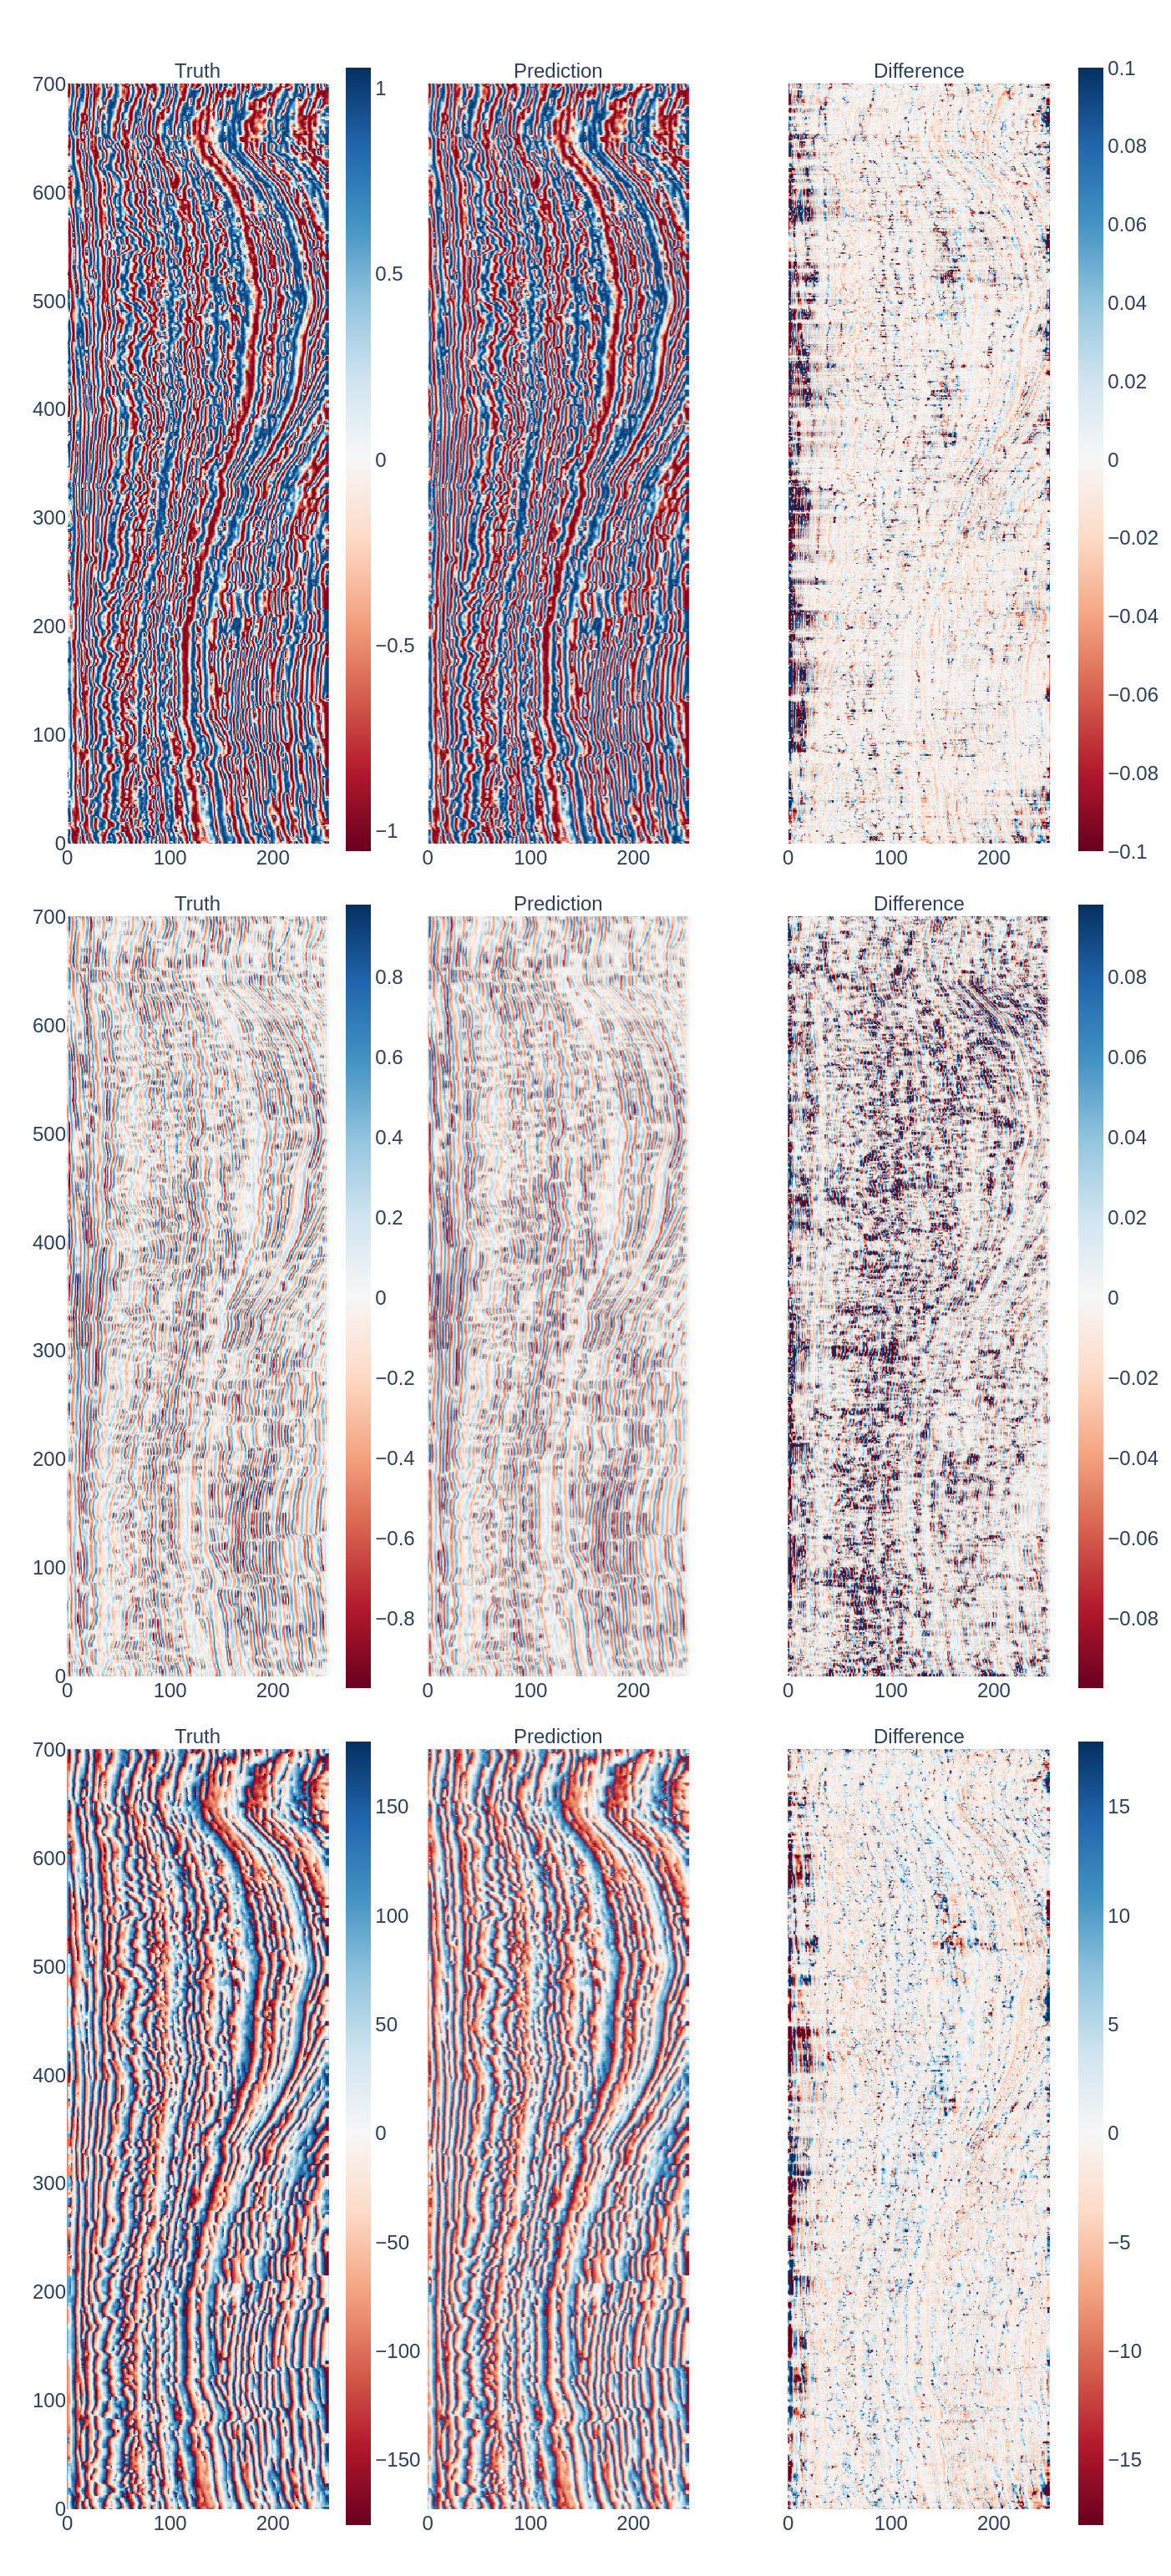
\includegraphics[width=1.0\columnwidth]{Fig/diferencas2.png}
%     \caption{Three inferred attributes, Cosine Instantaneous Phase, Amplitude Acceleration and Instantaneous Phase, and the difference between them and their ground truth. The difference scale is given by one tenth of the ground truth scale, since this is an acceptable value for the model error. In this way, it is easier to identify the points of greatest difficulty for each attribute. The abscissas of each graph are the depth while the ordinates are the crosslines} % remover ultimo comentario se adicionado nas imagens
%     \label{fig:diferencas}
% \end{figure}
%\begin{figure}[ht]
%    \centering
%    \includegraphics[width=1.0\columnwidth]{Fig/linha2.png}
%    \caption{First seismic trace of inline $2$ of the Frequency Change attribute from a depth of $100$. A big error in the prediction curve.}
%    \label{fig:fline}
%\end{figure}
%
%\begin{figure}[ht]
%    \centering
%    \includegraphics[width=1.0\columnwidth]{Fig/line.png}
%    \caption{First seismic trace of inline $2$ of the Cosine Instantaneous Phase attribute from a depth of $100$. Unlike the previous attribute, the prediction is almost completely coincident with the ground truth line, except for a few stretches where the distance between both is very small.}
%    \label{fig:cline}
%\end{figure}
%
%\begin{figure}[ht]
%    \centering
%    \includegraphics[width=1.0\columnwidth]{Fig/envelopeLine.png}
%    \caption{First seismic trace of inline $2$ of the Envelope attribute from a depth of $100$.}
%    \label{fig:eline}
%\end{figure}
%
%\begin{figure}[ht]
%    \centering
%    \includegraphics[width=1.0\columnwidth]{Fig/instantaneousPhaseLine.png}
%    \caption{First seismic trace of inline $2$ of the Instantaneous Phase attribute from a depth of $100$.}
%    \label{fig:iline}
%\end{figure}
\iffalse
\begin{figure*}[!t]
     \centering
     \begin{subfigure}[b]{0.49\textwidth}%1.0\columnwidth
        %\centering
        \includegraphics[width=1.0\columnwidth]{Fig/FrequencyChangeLine.png}
        \caption{
        %First seismic trace of inline $2$ of the Frequency Change attribute from a depth of $100$. A big error in the prediction curve.
        Frequency Change.}
        \label{fig:fline}
     \end{subfigure}
     \begin{subfigure}[b]{0.49\textwidth}%1.0\columnwidth
        %\centering
        \includegraphics[width=1.0\columnwidth]{Fig/CosineInstantaneousPhaseLine.png}
        \caption{
        Cosine Instantaneous Phase.
        %First seismic trace of inline $2$ of the Cosine Instantaneous Phase attribute from a depth of $100$. %Unlike the previous attribute, the prediction is almost completely coincident with the ground truth line, except for a few stretches where the distance between both is very small.
        }
        \label{fig:cline}
     \end{subfigure}
     %\hfill
     
     \begin{subfigure}[b]{0.49\textwidth}%1.0\columnwidth
        %\centering
        \includegraphics[width=1.0\columnwidth]{Fig/envelopeLine.png}
        \caption{
        %First seismic trace of inline $2$ of the Envelope attribute from a depth of $100$.
        Envelope.}
        \label{fig:eline}
     \end{subfigure}
     \begin{subfigure}[b]{0.49\textwidth}%1.0\columnwidth
        %\centering
        \includegraphics[width=1.0\columnwidth]{Fig/instantaneousPhaseLine.png}
        \caption{
        %First seismic trace of inline $2$ of the Instantaneous Phase attribute from a depth of $100$.
        Instantaneous Phase}
        \label{fig:iline}
     \end{subfigure}
       \caption{First seismic trace of inline $2$ for selected attributes from a depth of $100$.}
        \label{fig:examples}
\end{figure*}
\fi
\iffalse
\Cref{fig:xygraphic_all} illustrates the influence of the ground truth amplitude magnitude of the signal in the error performance.
An ideal regression line $x=y$ (predicted and analytical attributes are identical) and a linear regression line are shown in the figure. 
%built for the points and compared with the , in which the predicted attribute is identical to the analytical attribute.
The Envelope attribute presented a linear behavior with a small variance for the  \Cref{fig:xygraphic2}, confirming the low error values illustrated with the performance metrics.
Conversely, the Frequency Change, which was the worst attribute in the  R2 score, presents a large variance and divergence.
\fi
%\begin{figure}[ht]
%    \centering
%    \includegraphics[width=1.0\columnwidth]{Fig/relation.png}
%    \caption{Behavior of points predicted by the network compared to analytical attributes for Cosine Instantaneous Phase amplitude. It is possible to see that the linear regression line of the points is on the ideal line, which indicates a perfect prediction for this attribute. The few errors that occur are symmetric with respect to the identity line.}
%    \label{fig:xygraphic2}
%\end{figure}
%
%\begin{figure}[ht]
%    \centering
%    \includegraphics[width=1.0\columnwidth]{Fig/relation2.png}
%    \caption{Behavior of points predicted by the network compared to analytical attributes for Frequency Change amplitude. It is possible to see that the variance is very high, but the points still follow a linear trend. This trend has a smaller slope than the identity line, indicating that the model errs to a smaller module for very large amplitudes.}
%    \label{fig:xygraphic}
%\end{figure}%https://pt.overleaf.com/project/64440ce2d43590628f1e6947

% \begin{figure}[!t]
%      \centering
%      \begin{subfigure}[b]{0.49\textwidth}%1.0\columnwidth
%         \includegraphics[width=1.0\columnwidth]{Fig/relation.png}
%         \caption{Cosine Instantaneous Phase. 
%         %Behavior of points predicted by the network compared to analytical attributes for Cosine Instantaneous Phase amplitude. It is possible to see that the linear regression line of the points is on the ideal line, which indicates a perfect prediction for this attribute. The few errors that occur are symmetric with respect to the identity line.
%         }
%         \label{fig:xygraphic2}
%      \end{subfigure}
     
%      \begin{subfigure}[b]{0.49\textwidth}%1.0\columnwidth
%         \includegraphics[width=1.0\columnwidth]{Fig/relation2.png}
%         \caption{Frequency Change.
%         %Behavior of points predicted by the network compared to analytical attributes for Frequency Change amplitude. 
%         %It is possible to see that the variance is very high, but the points still follow a linear trend. This trend has a smaller slope than the identity line, indicating that the model errs to a smaller module for very large amplitudes.
%         }
%         \label{fig:xygraphic}
%      \end{subfigure}
%      \caption{Ground Truth vs Predicted Values}
%     \label{fig:xygraphic_all}
% \end{figure}


% In order to try to understand if the raw error was relevant for the model performance and thus identifying possible causes of higher MSE metrics, it is necessary to look at the relative error, that is, a ratio between the ground truth data and the predicted data \Cref{fig:ratio_all}. %\Cref {fig:ratio} and \Cref{fig:ratio2}.
% %
% Although the modulus of the predicted values of Frequency Change is smaller than that of the ground truth values, the relative error decreases as the modulus increases. Furthermore, as the amplitude approaches zero, the model becomes very unstable, varying its relative error a lot. This must happen because the calculation depends on neighboring amplitudes (\Cref{fig:examples}).
% Conversely, this ratio for the Cosine Instantaneous Phase is almost constant around 1. The high ratios close to $0$ are expected because the numerator of the ratio is a small number close to zero.

        
%\begin{figure}[ht]
%    \centering
%    \includegraphics[width=1.0\columnwidth]{Fig/ratio3.png}
%    \caption{Here it is possible to see that although the modulus of the predicted values of Frequency Change is smaller than that of the ground truth values, the relative error decreases as the modulus increases. Furthermore, as the amplitude approaches zero, the model becomes very unstable, varying its relative error a lot. This must happen because the calculation depends on neighboring amplitudes, as you can see in figure \ref{fig:linha}}
%    \label{fig:ratio}
%\end{figure}
%
%\begin{figure}[ht]
%    \centering
%    \includegraphics[width=1.0\columnwidth]{Fig/ratio.png}
%    \caption{Ratio between ground truth and prediction for Cosine Instantaneous Phase. It is possible to verify a constancy in the error percentage. The error close to $0$ is expected due to the numerator of the fraction being zeroed, causing instability}
%    \label{fig:ratio2}
%\end{figure}

% \begin{figure}[!t]
%      \centering
%      \begin{subfigure}[b]{0.49\textwidth}%1.0\columnwidth
%         \includegraphics[width=1.0\columnwidth]{Fig/ratio3.png}
%         \caption{
%         %Here it is possible to see that although the modulus of the predicted values of Frequency Change is smaller than that of the ground truth values, the relative error decreases as the modulus increases. Furthermore, as the amplitude approaches zero, the model becomes very unstable, varying its relative error a lot. This must happen because the calculation depends on neighboring amplitudes, as you can see in \Cref{fig:linha}
%         Frequency Change.
%         }
%         \label{fig:ratio}
%      \end{subfigure}
     
%      \begin{subfigure}[b]{0.49\textwidth}%1.0\columnwidth
%         \includegraphics[width=1.0\columnwidth]{Fig/ratio.png}
%         \caption{
%         Cosine Instantaneous Phase. 
%         %Ratio between ground truth and prediction for Cosine   Instantaneous Phase. It is possible to verify a constancy in the error percentage. The error close to $0$ is expected due to the numerator of the fraction being zeroed, causing instability
%         }
%         \label{fig:ratio2}
%      \end{subfigure}
%      \caption{Ground Truth/Prediction Ratio}
%     \label{fig:ratio_all}
% \end{figure}

% Além desses resultados é possível verificar também a curva de aprendizado. Todas possuiram um treinamento muito cedo (próximo a época 25 todas as loss se estabilizaram próximo ao zero), com a validation loss and training loss muito próximas. Apenas uma possuiu um comportamento diferente, a curva do atributo Intantaneous phase, que está apresentada na figura \ref{fig:loss}. A figura mostra um sinal de overfiting com início na época $25$. Ao final das 200 épocas o erro de treinamento foi de $45$ enquanto o erro  de validacao foi de $490$. A curva da validação atinge o menor erro de $413$ na época $59$.

% In addition to these results, it was also possible to verify the learning curve. They all had very early training (close to the $25$ epoch, all losses stabilized close to zero, similar to \Cref{fig:loss2}), with the validation loss and training loss very close. Only one had a different behavior, the curve of the Instantaneous phase attribute \Cref{fig:loss}, which suffered from over-fitting signal starting at the $25$ epoch. At the end of the $200$ epochs, the training error was $45$ while the validation error was $490$. The validation curve reaches the smallest error of $413$ at the time $59$.

%\begin{figure}[ht]
%    \centering
%    \includegraphics[width=1.0\columnwidth]{Fig/loss2.png}
%    \caption{Learning curve considering the MSE loss function for envelope}
%    \label{fig:loss2}
%\end{figure}
%
%\begin{figure}[ht]
%    \centering
%    \includegraphics[width=1.0\columnwidth]{Fig/loss.png}
%    \caption{Learning curve considering the MSE loss function for instantaneous phase}
%    \label{fig:loss}
%\end{figure}

% \begin{figure}[!t]
%      \centering
%      \begin{subfigure}[b]{0.49\textwidth}%1.0\columnwidth
%          \includegraphics[width=1.0\columnwidth]{Fig/loss2.png}
%         \caption{Envelope}
%         \label{fig:loss2}
%      \end{subfigure}
     
%      \begin{subfigure}[b]{0.49\textwidth}%1.0\columnwidth
%         \includegraphics[width=1.0\columnwidth]{Fig/loss.png}
%         \caption{Instantaneous Phase}
%         \label{fig:loss}
%      \end{subfigure}
%      \caption{Learning curve considering the MSE loss function}
%     \label{fig:loss_all}
% \end{figure}

\subsection{Limitations}

%A partir desses resultados é possível verificar que a rede possui uma grande capacidade de aprendizado em relação a predição de atributos sísmicos. Ainda assim é possível verificar um erro acontecendo em diversos atributos, os quais podem ou não ser relevantes para os geólogos, geofísicos ou ainda outras redes neurais que tentem realizar a segmentação semantica das fáceis sísmicas através desses atributos.
%Dessa forma torna-se necessário uma rede ainda mais complexa como as GANs ou transformers.

It was evinced that the trained models have a great learning capacity for predicting a seismic attribute. However, prediction errors occur for some attributes, particularly, for instantaneous phase and \lbp. The latter is a 3D attribute and may require neighborhood information to improve the model prediction performance. This information, however, is not fully captured with the 2D model employed in this study. 

It is still not clear whether these errors are relevant to geologists, geophysicists, or even to other neural network models performing a task that employs an attribute as input, for instance, semantic segmentation of seismic facies \cite{semantic-segmentation}. Thus, the impact of the observed errors on tasks in which the attributes are employed deserves further analysis. If the performance of this CNN model is not enough for a given application, thus, more complex techniques to attribute calculation may be still necessary, such as 3D CNN models, GANs \cite{SEG20-navarro-seismic-attr} or transformers \cite{transformers}.

%Além disso esse trabalho não utilizou tamanhos diversos no treinamento dos modelos, o que exige um recorte das imagens de treino e teste nas mesmas dimensões. Essas dimensões definem também o gasto de memória da rede, uma vez que ela não realiza o tratamento das imagens em janelas, tendo como entrada o dado completo. Dados grandes ainda podem ser preditos desde que realizado o recorte e preprocessamento adequado antes.

% In addition, this work employed a single input size in the training of the models. To support different input sizes, training and test images must be clipped to the same dimensions. These dimensions also define the model memory consumption, since it does not process the images in windows, having as input the complete data. Large data can still be predicted as long as proper clipping and preprocessing is performed first.

%Também não foram testados dados e atributos extraidos de outras regiões geográficas diferentes do F3, o que pode ser gerar uma limitação no aprendizado da rede que não foi verificado.

% Finallyy, Data and attributes extracted from other geographic regions other than F3 were also not tested, which may generate a limitation in the learning of the network that was not verified.

\section{Conclusion}
\label{sec:conslusion}
%Nesse estudo foi possível verificar a possibilidade da utilização da rede neural convolucional Unet como forma de gerar atributos sísmicos muito semelhantes aos atributos calculados matematicamente. A rede pontua diferentemente para cada atributo sísmico, de forma geral produzindo resultados melhores para atributos contínuos, como envelope, e resultados levemente piores como a fase instantanea. A diferença entre a inferencia e o grond truth não pode ser identificada visualmente sem um destaque como o cálculo das differenças entre as imagens, mas esse erro pode ser relevante quando se trata de outras redes neurais predizendo as fáceis ou horizontes sísmicos. 

This work has demonstrated the feasibility of using the \unet convolutional neural network to calculate seismic attributes, whose outputs are very similar to those calculated mathematically. The network scores differently for each seismic attribute, producing generally better results for continuous attributes, such as envelope, and slightly worse results for instantaneous phase and \lbp. In many cases, the difference between the inference and the ground truth cannot be visually identified without some help, such as the calculation of the differences between the images. It is necessary to understand whether this error is relevant for tasks employing the attributes, such as neural networks to predict seismic facies or horizons.

%Há ainda uma necessidade de mais dados no treinamento para alguns atributos, enquanto outros convergem muito rapidamente sem gerar overfitting. A velocidade de inferencia é a mesma independente do atributo treinado, o que é um bom indicativo para essa rede substituir o cálculo de atributos mais custosos.

%There is still a need for more training data for some attributes, while others converge very quickly without over fitting. The inference speed is the same regardless of the trained attribute, which is a good indication for this network to replace the calculation of more costly attributes.

%Some attributes still require additional training data, while others converge rapidly without overfitting.
The constant inference speed of the CNN regardless of the trained attribute being calculated is a strong motivation to train deep learning models to replace the calculation of seismic attributes, especially those more expensive computationally.

\section{Acknowledgments}
%This work was supported by Petrobras.
We would like to thank PETROBRAS for funding this study and %. % and for permission to publish this work.
SENAI/CIMATEC for providing access to supercomputing resources. Prof. Borin also received funding from CNPq (314645/2020-9, 404087/2021-3) and Fapesp (2013/08293-7).
\balance
\bibliographystyle{plain} % We choose the "plain" reference style
\bibliography{paper}


\end{document}
